% chapter 5 section 2

\section{原子模型}

\subsection{电子的发现}

在空气稀薄的玻璃管两端施加高电压后,可在管内发现放电而产生的发光现象。进一步抽去管内气体后,发光现象消失,但可在玻璃管的正极侧发现亮斑。
\begin{figure}[ht!]
    \centering
    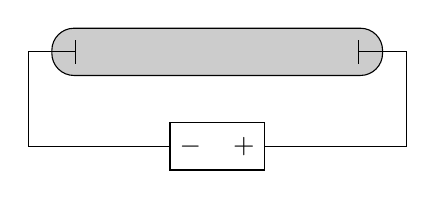
\begin{tikzpicture}[scale=0.6]
        \draw (0,0) rectangle (2,1);
        \draw (2,0.5) node[left] {$+$} -- (5,0.5) -- (5,2.5) -- (4,2.5);
        \draw (4,2.75) -- (4,2.25);
        \draw (0,0.5) node[right] {$-$} -- (-3,0.5) -- (-3,2.5) -- (-2,2.5);
        \draw (-2,2.75) -- (-2,2.25);
        \filldraw[rounded corners=8pt, fill=gray, color=black, fill opacity=0.2] (-2.5,2) rectangle (4.5,3);
    \end{tikzpicture}
    \caption{真空放电}
\end{figure}
这种现象就像是有什么物质从负极射出后击打到了正极侧一样,所以当时人们将其命名为阴极射线。并发现阴极射线具有如下的性质。
\begin{itemize}
    \item 在无外界影响的环境下其运动轨迹为直线。
    \item 在空间中施加电场或是磁场后其运动轨迹会发生偏移。
    \item 击打到物体上之后会有一定的压力作用。
    \item 上述性质与极板金属和玻璃管内气体无关。
\end{itemize}
因此人们断定阴极射线是实物粒子且带有负电,后命名为电子。

\subsection{有核模型}

\subsubsection{初期猜想}

1897年JJ汤姆孙(英国)发现了电子,并提出了原子的枣糕模型,即电子均匀地分布在带有正电的球中。尽管这种无核模型在某种程度上可以解释原子的稳定性的问题,但却无法说明原子质量的问题。1908年汤姆孙的学生卢瑟福(新西兰)通过其著名的$\alpha$粒子轰击金箔的实验\footnote{如果原子无核,那么质量远大于电子的$\alpha$粒子在穿过原子时理应只发生小幅度的偏移,虽然大部分实验现象皆是如此,但仍然存在极少的$\alpha$粒子发生了巨大的偏移,即原子内存在$\alpha$粒子也无法撼动的极重物质。}发现了原子核的存在,从而确立了有核模型的正确性。

然而,卢瑟福(新西兰)的模型仍非完美。倘若电子在围绕着原子核不停地转动,那么势必会形成环形电流,进而形成磁场。磁场的变化再次激发出电场,如此往复则会释放出电磁波,最终使得电子的能量在不断地减少。也就是说电子并非处于一个安定的状态,原子也非安定。对此尼尔斯波尔(丹麦)于1913年给出了解决方案。

\subsubsection{波尔模型}

\paragraph{波尔假说} 波尔认为原子核周围存在\underline{能级},核外电子只会处于各个能级上,并且是稳定的。同时,这些能级从物质波的角度可以理解为电子在特定轨道上形成了驻波,从而稳定存在。
\begin{figure}[ht!]
    \centering
    \begin{tikzpicture}[scale=1]
        \draw (0,0) circle (1);
        \fill (0,0) circle (0.1);
        \foreach \a in {0,...,360}
            \fill ($({cos(\a)},{sin(\a)}) + (\a:{0.3*sin(8*\a)})$) circle (0.5pt);
    \end{tikzpicture}
    \caption{波尔模型}
\end{figure}
因此只有轨道周长是电子波长的整数倍时才能够实现,并将这个条件称为\underline{量子条件}
\begin{equation*}
    2\pi r=n\lambda=n\cdot\frac{h}{mv}
\end{equation*}

\paragraph{氢原子轨道半径} 有核模型下电子围绕原子核做等速圆周运动,以库仑力作为向心力,因此
\begin{equation*}
    m\frac{v^2}{r}=k\frac{e^2}{r^2}
\end{equation*}
再结合量子条件可得
\begin{equation*}
    r_n=\frac{h^2}{4\pi^2kme^2}n^2
\end{equation*}
由此可见氢原子的轨道半径的确是随着整数$n$而离散变化的,而这些离散的轨道正是化学中所提及的电子壳层(KLM等)。

\paragraph{氢原子能级} 基于电子运动的动能以及库仑力作用下的电势能可求出每一能级下电子的能量
\begin{equation*}
    E=\frac12mv^2+k\frac{-e^2}{r}=-\frac{ke^2}{2r}
\end{equation*}
再代入轨道半径可整理得到
\begin{equation*}
    E_n=-\frac{2\pi^2k^2me^4}{h^2}\times\frac{1}{n^2}
\end{equation*}
可见氢原子的每个能级所对应的能量也是随着整数$n$而离散变化的。并且一般情况下电子会选择处于能量更小的能级,也就是所谓的\underline{基态}(基底状態),同时称非基底状态为\underline{激发态}(励起状態)。由能级公式可知,不同能级间的能量差为定值
\begin{equation*}
    E_m-E_n=\frac{2\pi^2k^2me^4}{h^2}\left(\frac{1}{n^2}-\frac{1}{m^2}\right)
\end{equation*}
因此,当核外电子从激发态回归到基态时只会释放出能量等同于两个能级能量差的光子,即
\begin{equation*}
    E_m-E_n=h\nu
\end{equation*}
相反,只有能量等于两个能级能量差的光子才会使处于基态的电子转移到对应的激发态。一般称这个过程为\underline{跃迁}。

虽然得益于波尔的猜想合理解释了关于氢原子的诸多疑点,比如其吸收光谱不连续等问题,但原子层面的问题却并未因此尘埃落定。事实上,该猜想只能够完美说明氢原子的情况,对于更加普遍也更加复杂的其他原子就有些力不从心了。

\subsection{放射性衰变}

\begin{figure}[ht!]
    \centering
    \begin{minipage}[c]{0.48\textwidth}
        \centering
        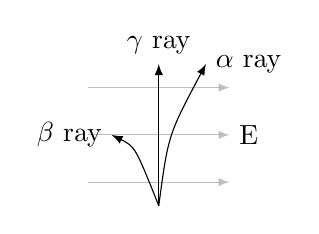
\begin{tikzpicture}[scale=0.6]
            \foreach \y in {0,1,2}
                \draw[-latex,color=gray,opacity=0.5] (0,\y) -- (3,\y);
            \node[right] at (3,1) {E};
            \draw[-latex] (1.5,-0.5) ..controls(1.7,1).. (2.5,2.5) node[right] {$\alpha$ ray};
            \draw[-latex] (1.5,-0.5) ..controls(1,0.75).. (0.5,1) node[left] {$\beta$ ray};
            \draw[-latex] (1.5,-0.5) -- (1.5,2.5) node[above] 
            {$\gamma$ ray};
        \end{tikzpicture}
    \end{minipage}
    \begin{minipage}[c]{0.48\textwidth}
        \centering
        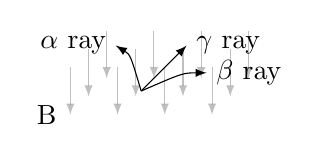
\begin{tikzpicture}[scale=0.6]
            \foreach \x in {0.5,1.5,2.5,3.5} \foreach \z in {0.5,1.5,2.5}
                \draw[-latex,color=gray,opacity=0.5] (\x,0.5,\z) -- (\x,-0.5,\z);
            \node at (0,-0.5,2.5) {B};
            \draw[-latex] (2,0,2.5) ..controls(1,0,0.5).. (0.5,0,0) node[left] {$\alpha$ ray};
            \draw[-latex] (2,0,2.5) ..controls(2.5,0,1.5).. (3,0,1.5) node[right] {$\beta$ ray};
            \draw[-latex] (2,0,2.5) -- (2,0,0) node[right] {$\gamma$ ray};
        \end{tikzpicture}
    \end{minipage}
    \caption{放射线}
\end{figure}
处于不稳定状态的原子核通过放射粒子或是能量后变得稳定的过程为衰变(radioactive decay),大体有三种典型衰变模式。
\begin{figure}[ht!]
    \centering
    \renewcommand\arraystretch{1.2}
    \begin{tabular}{c|c|c|c}
        \hline
        &本质&穿透力&电离效果\\\hline
        $\alpha$衰变&\ce{^4_2He}原子核&低&高\\\hline
        $\beta$衰变&高速\ce{^0_{-1}e}&中&中\\\hline
        $\gamma$衰变&高能电磁波&高&低\\\hline
    \end{tabular}
    \caption{衰变一览}
\end{figure}
计算时可先使用前后质量只差算出$\alpha$衰变的次数,而后使用$\beta$衰变补全电荷的数量。
\begin{itemize}
    \item \ce{^226_88Ra -> ^222_86Rn + ^4_2He}
    \item \ce{^210_83Bi -> ^210_84Po + ^0_-1e-}
\end{itemize}
此外,一般用\underline{半衰期}来描述衰变的发生速度,即每过一个半衰期原子核的数量便会减少一半。
\begin{figure}[ht!]
    \centering
    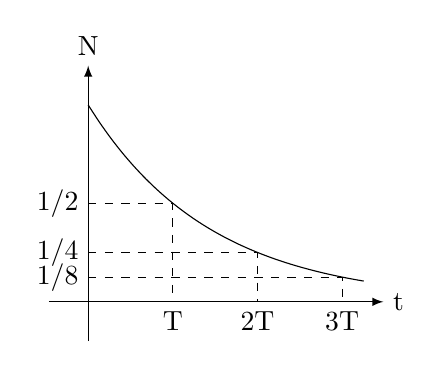
\begin{tikzpicture}[scale=2.5]
        \draw[-latex] (-0.2,0) -- (1.5,0) node[right] {t};
        \draw[-latex] (0,-0.2) -- (0,1.2) node[above] {N};
        \draw[domain=0:1.4] plot[smooth] (\x,{0.2^\x});
        \draw[dashed] (0,1/2) node[left] {1/2} -| (0.43,0) node[below] {T};
        \draw[dashed] (0,1/4) node[left] {1/4} -| (0.86,0) node[below] {2T};
        \draw[dashed] (0,1/8) node[left] {1/8} -| (1.29,0) node[below] {3T};
    \end{tikzpicture}
    \caption{半衰期}
\end{figure}

\subsection{核能}

守恒一直是物理学家们的执着,和对称性一样被认为是自然的美。然而,随着粒子研究的深入,人们惊异地发现在原子核的层面上出现了质量不守恒的现象。即构成原子核和核子的总质量小于原子核所表现出的质量,并称该现象为\underline{质量亏损}。

在此爱因斯坦(美国)提出质量和能量的等价性,由此将质量守恒和能量守恒统一在了一起。
\begin{equation*}
    E=mc^2
\end{equation*}
此外,从物质的稳定性的角度也可以解释质量亏损的现象:物质总会自发地向能量低(稳定)的状态发展,因此不稳定的核子结合为稳定的原子核后能量(质量)会降低。
